\documentclass[a4paper,12pt,final,oneside,openright]{article}
\usepackage{report}

\newcommand{\reporttitle}{Statistical Methods in Applied Computer Science}
\newcommand{\enseignants}{
Jens~\textsc{Lagergren}}

\newcommand{\reportauthor}{
Rémi DOMINGUES}
% \newcommand{\hexanome}{H4211}
\newcommand{\reportsubject}{}
\newcommand{\stagetopic}{Project 2 - The magic word}
\newcommand{\dateperiod}{December $15^{th}$ - January $18^{th}$}
\newcommand{\HRule}{\rule{\linewidth}{0.5mm}}
\setlength{\parskip}{1ex} % Espace entre les paragraphes

\hypersetup{
    pdftitle={\reporttitle},%
    pdfauthor={\reportauthor},%
    pdfsubject={\reportsubject},%
    pdfkeywords={}
}

\title{\reporttitle}
\author{\reportauthor}

\setlongtables
\usepackage[font=small,skip=0pt]{caption}
\usepackage{algorithm}
\usepackage{algpseudocode}


%\setcounter{tocdepth}{4}
\begin{document}
    \renewcommand{\chaptername}{} %\renewcommand{\thechapter}{}
    \renewcommand{\contentsname}{Contents}

    \pagestyle{empty}
    \pagenumbering{arabic}
    % Inspiré de http://en.wikibooks.org/wiki/LaTeX/Title_Creation
\begin{center}
	\begin{minipage}[t]{0.48\textwidth}
	  \begin{flushleft}
	    
\includegraphics [width=30mm]{img/logo_kth.jpg} \\[0.1cm]
		Kungliga Tekniska Högskolan\\
		Valhallavägen 79\\
		100 44 Stockholm
	  \end{flushleft}
	\end{minipage}
	\begin{minipage}[t]{0.48\textwidth}
	  \begin{flushright}
	  \end{flushright}
	\end{minipage} \\[1cm]

	\textsc{\Large \reportsubject}\\[0.3cm]
	\HRule \\[0.4cm]
	{\Huge \bfseries \reporttitle}\\[0.3cm]
	{\LARGE \bfseries «~\stagetopic~»}\\[0.3cm]
	{\Large \dateperiod}\\[0.4cm]
	\HRule \\[1.5cm]

	
\includegraphics [width=0.7\linewidth]{img/icon.png} \\[1.5cm]
	\begin{minipage}[t]{0.5\textwidth}
	  \begin{flushleft} \large
	    \emph{Author}\\
	    \reportauthor
	  \end{flushleft}
	\end{minipage}
	\begin{minipage}[t]{0.4\textwidth}
	  \begin{flushright} \large
	    \emph{Teacher} \\
	    \enseignants
	  \end{flushright}
	\end{minipage}

	\vfill
	\footnotesize{Scholar year 2014-2015}
\end{center}

    \pagebreak
    \sloppy          % Justification moins stricte : des mots ne dépasseront pas des paragraphes

    %\frontmatter
    \thispagestyle{empty}
    %\tableofcontents
    \addtocontents{toc}{\protect\thispagestyle{empty}}
    \pagebreak

    %\mainmatter
    \pagestyle{headings}
    %\renewcommand{\chaptermark}[1]{\markboth{\MakeUppercase{\chaptername\ \thechapter.\ #1}}{}}
    %\renewcommand{\sectionmark}[1]{\markright{\thesection{} #1}}

    \section{Intro}
The aim of this project is to implement a \textbf{generator} which outputs \textbf{sequences} containing a \textbf{magic word}, and a \textbf{Gibbs sampler} which aims at finding the magic words in the previous sequences.

For this purpose, we generate N sequences $s_i$ of length M, each containing a magic word of length w. Our Gibbs sampler should find $R = {r_1,...,r_n}$ with $r_i$ the starting position of the magic word in the $i^{th}$ sequence.

The \textbf{background} of a sequence is the union of every observation in a sequence which does not belong to the magic word.

A \textbf{magic word} is the union in a sequence of every observation having its index \textit{i} between $r_i$ and $r_i + w - 1$.

The experiment described in this report will focus on finding this motif described by a Dirichlet prior related to an alphabet. We have chosen to apply our Gibbs sampler to DNA sequences. Therefore, the alphabet K is K = \{A, T, G, C\}.

\section{Generation}
The background and magic word have the same alphabet

We start by generating for each sequence the starting position $r_i$ of the magic word: $r_i = U(N-w+1)$


Then, we sample the background of each sequence:

\begin{equation}
s_{i,j} \sim Cat(x|\theta)
\end{equation}

With with $\theta \sim Dir(\theta|\alpha')$ and $s_{i,j}$ the letter \textit{j} in the sequence \textit{i}.


We also do the same for the magic words:

\begin{equation}
s_{i,k} \sim Cat(x|\theta_j)
\end{equation}

With $\theta \sim Dir(\theta_j|\alpha)$ and $k \in [r_i, r_i+w-1]$.
\\

$\alpha$ and $\alpha'$ are vectors of continuous reals, and parameters of our Dirichlet distributions which are multivariate probability distributions.

For our generation process, we define $\alpha' = (1,...,1)$ as a vector of same size as the alphabet K. The categorical distribution obtained from $Dir(\alpha)$ will here contain a lot of randomness, since we do not specify a higher weight for any letter of the alphabet. However, all sequences will be generated from the same categorical distribution. If using a $\alpha$ different enough from $\alpha'$, we should thus be able to decide whether a sequence of letters has been generated from $Dir(\alpha)$ or $Dir(\alpha')$.

We will use various $\alpha$, parameter for the magic word generation, during this experiment. The tricky part in the inference process is that each letter in a given magic word is generated using distinct samples from $Dir(\alpha)$, giving us distinct categorical distributions. This should add more randomness to our words, and therefore will require more data to give an accurate $r_i$. Let us precise however that every word will be generated from the same set of categorical distributions (one distribution for each letter).

The code of the generator is written in \textit{generator.py}


\section{Inference}
Our goal is now to implement a Gibbs sampler in order to estimate the posterior $P(R|D)$ with $R = {r_1,...,r_N}$ and $D = {s_1,..,s_N}$.

Each state of our Gibbs sampler will be a $\widehat{R_i}$ with $\widehat{R_i} = {\widehat{r_{i,1}},..,\widehat{r_{i,N}}}$. Finding those steps by iterating is the aim of the Markov Chain Monte Carlo algorithm described here.

Please note that $\alpha$ and $\alpha'$ are given to our algorithm.
\\

To simplify to computation of the posteriors, we use a collapsed Gibbs sampler, i.e. we collapse the Dirichlet distribution $Dir(\theta_j|\alpha)$ which has been used as prior to generate our categorical distributions $Cat(x|\theta_j)$.
Collapsing our Gibbs sampler will introduce a dependences between those categorical distributions.
\\

In order to get a better accuracy for our results, we must also pay attention to the \textit{burn-in period} and the correlation between a state (a $R_i$ in the Markov Chain generated by our Gibbs sampler) and its child. Thus, once this Markov Chain generated, the first S steps (\textit{burn-in period}) must be ignored since the stationary distribution has not been reached yet by our algorithm, giving unstable results until we reach a convergence.

Then, we must build our final results by aggregating every $i^{th}$ state after the state $R_S$. Keeping a certain number of steps between each considered for the results should lower the impact of the correlation between the states, and improve the final accuracy.
\\

The implementation follows the shema below:

\begin{algorithmic}[1]
\State \Comment Gibbs sampling
\State Generate randomly $R_0$
\For{i from 0 to NITER}
    \For{j from 0 to NSEQUENCES}
            \State $P(\widehat{r}_{i_j}|\widehat{R}_{i_{-j}}, D) = \cup_{l = 0}^{M-w} P(D_{background}|\widehat{R}_{i_{-j}},\alpha') \prod\limits_{k = l}^{l + w} P(D_{motif_k}|\widehat{R}_{i_{-j}},\alpha)$
        \State $\widehat{r}_{i_j} = sample(P(\widehat{r}_{i_j}|\widehat{R}_{i_{-j}},D))$ \Comment $\widehat{r}_{i_j}$ is generated from the categorical $P(\widehat{r}_{i_j}|\widehat{R}_{i_{-j}},D)$
    \EndFor
\EndFor

\State \Comment Results sampling from the Markov chain generated by the Gibbs sampler
\For{i from 0 to NSEQUENCES}
    \State seq = sequences[i]
    \State $\widehat{r}_i = argmax(count_{t = S:k:NITER}(\widehat{R}_{t_i}))$ \Comment We select the starting index which has been the most elected for a sequence. Only the $k^{th}$ results after the \textit{S} first states are taken into account (steps from S to N with a step size of k)
\EndFor
\end{algorithmic}

With

\begin{equation}
P(D_{background}|\widehat{R}_{i_{-l}},\alpha') = \frac{\Gamma (\sum\limits_{k = 1}^{|K|} \alpha_k')}{\Gamma (|K|(M-w) + \sum\limits_{k = 1}^{K} \alpha_k')} \prod\limits_{k = 1}^{|K|} \frac{\Gamma(B_k + \alpha_k')}{\Gamma(\alpha_k')}
\end{equation}

and

\begin{equation}
P(D_{motif_j}|\widehat{R}_{i_{-l}},\alpha) = \frac{\Gamma (\sum\limits_{k = 1}^{|K|} \alpha_k)}{\Gamma (|K| + \sum\limits_{k = 1}^{|K|} \alpha_k)} \prod\limits_{k = 1}^{|K|} \frac{\Gamma(N_k + \alpha_k)}{\Gamma(\alpha_k)}
\end{equation}

Where $|K|$ is the length of the alphabet K, $B_k$ is the number of times the symbol $K_k$ appears in the background, and $N_k$ is the number of times the symbol $K_k$ appears in the given column \textit{j} of the motif.

Therefore, the equation in line 4 returns a categorical from which we sample a starting position $\widehat{r}_{i_l}$ for the $i^{th}$ state for the sequence \textit{l}.
This is done by computing equations 3 and 4 for every possible value $\widehat{r}_{i_l}$ in a range from 0 to M-w-1, i.e. by using $\widehat{R}_i$ with various $\widehat{r}_{i_l}$.

The implementation of this algorithm can be found in \textit{gibbs\_sampler.py}


\section{Testing}
The performances depend on the whether the differences between $\alpha$ and $\alpha'$ are important or not. Obviously, if one of the $\alpha_i$ is really high, we are more likely to detect the magic word with high accuracy.

With $\alpha' = (1,...,1)$ and $\alpha = (1,7,10,2)$, we can observe the following results (5 sequences of length 30 with a magic word of length 10, sample selection with 200 iterations, every $10^{th}$ iteration from the $100^{th}$):

\begin{figure}[H]
\centering
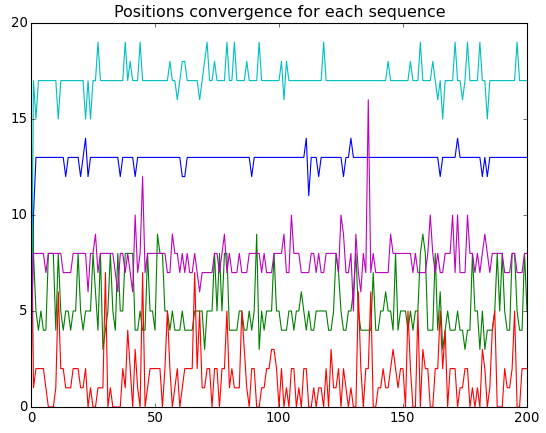
\includegraphics[width=0.7\linewidth]{img/c.png}
\caption{Starting position (vertical axis) for each sequence (function) - 40\% accuracy}
\end{figure}

We can observe quite stable results. However, the the \textit{burn-in} period seems nonexistent with an immediate convergence. For the previous chart we had an accuracy of 40\%. The real positions were [13, 8, 2, 17, 11] and the positions found [13, 4, 0, 17, 8].

We must remind also that an accuracy of 40\% means that we have found 40\% of the correct starting positions among $N * (M - w)$ positions, so we found for example 2 correct positions among the 5 real positions in a set of 150 positions, which is still really nice, considering that a wrong position can be very close to the real position, and be misleaded because of an unlucky sequence generation.

Those results are highly dependent on the sequence sampling, since it can be hard sometimes to find when a magic word starts. Below is another example for the same parameters:

\begin{figure}[H]
\centering
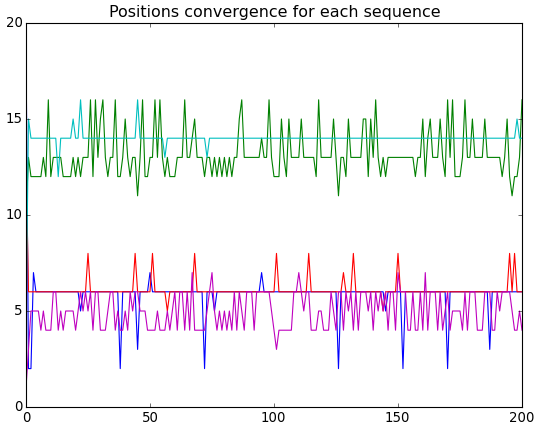
\includegraphics[width=0.7\linewidth]{img/e.png}
\caption{Starting position (vertical axis) for each sequence (function) - 60\% accuracy}
\end{figure}

60\% accuracy were found here, with the real positions [6, 12, 6, 14, 5] and the estimated positions [6, 13, 6, 14, 4] (with 13 and 4 really close to the real positions 12 and 5).

Using a \textbf{higher number of sequences} or a \textbf{$\alpha$ and $\alpha'$ more different} could therefore lead to better results.
\\


We now use \textbf{$\alpha = (1,7,20,2)$}, increasing the difference between $\alpha$ and $\alpha'$ to ease the identification:

\begin{figure}[H]
\centering
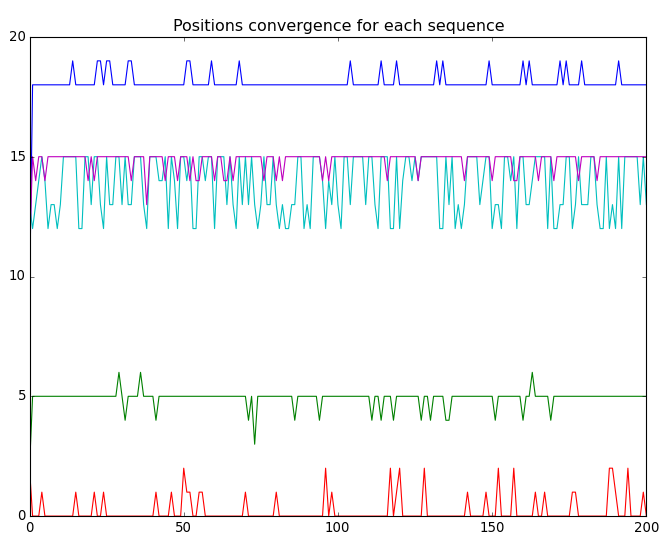
\includegraphics[width=0.7\linewidth]{img/b.png}
\caption{Starting position (vertical axis) for each sequence (function) - 100\% accuracy}
\end{figure}

100\% accuracy is now observed for the starting positions [18, 5, 0, 12, 15].
\\

However, our performances also depend on the parameters chosen for our samples selection among the states generated by our Gibbs sampler.
The \textit{number of iterations} is the number of states generated, \textit{min\_step} is the length of the \textit{burn-in period} and \textit{step\_size} determines the number of steps between each state taken into account for our results (all of these steps are between \textit{min\_step} and the total \textit{number of iterations}).

They also depend on the parameters selection for \textit{N, M} and \textit{w}. Below are various benchmarks for $M = 20$:

\begin{figure}[H]
\centering
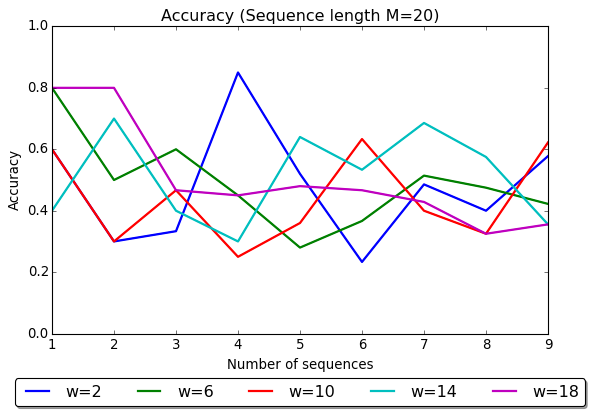
\includegraphics[width=0.7\linewidth]{img/tests.png}
\caption{Benchmarks for various N and w for $M = 20$}
\end{figure}

Nevertheless, we can hardly infer any trend and certainty from those functions. Indeed, despite of running the estimation for 5 different sampling for a given N and w, no trend can be observed here.

However, we can at least see that using more sequences should make our results more stable. Theorically, if we had not run the sampling multiple times for a given configuration, we should also have had better and more stable results since we make our Gibbs sampler more resistant to the randomness induced when sampling our sequences.

For more details, the testing implementation is written in \textit{testing.py}


    %\backmatter
\end{document}
